\documentclass[12pt,letter]{article}
\usepackage[moduleName={Name Corp Octal Wave Generator}]{KautenjaDSP}
% import a debugging package to show the margin boxes
% \usepackage{showframe}
% set the graphics path to the img directory
\graphicspath{{img/}}

% algorithm2e stuff
% \SetKwInOut{Objects}{$\CKmatrix{O}$}
% \SetKwInOut{Weights}{$\CKvector{w}$}

\begin{document}
\titlePage{Logo}{Module}{KautenjaDSP}

% -------------------
% MARK: Overview
% -------------------

\section{Overview}

106 is an emulation of the Namco 106 audio processing unit from the Nintendo Entertainment System (NES) for VCV Rack. The Namco 106 chip contains eight wave-table oscillators and 128 bytes of operational RAM for wave-table data. The wave-tables are 4-bit and can be as long as 63 samples. This module uses a bank of five 32-sample wave-tables to act as the waveform for all eight oscillators.

Namco 106 provides the key features of the Namco 106 chip, namely,
\begin{itemize}
  \item \textbf{Wave-table synthesis:} 8 wave-table oscillators with sample bit depth of 4 bits and wave-table size of 32 samples
  \item \textbf{Waveform morph:} 5 banks of wave-tables to morph between using 32-bit floating point linear interpolation (not very retro, but it sounds nice)
  \item \textbf{Frequency control:} 18-bit frequency control with linear frequency modulation
  \item \textbf{Amplitude modulation:} 4-bit amplifier with linear amplitude modulation
  \item \textbf{Namco 106 compute limitation:} activating each additional oscillator (up to 8) reduces the amount of compute available for all oscillators. This causes all oscillators to drop in frequency when additional oscillators are activated.
\end{itemize}

% -------------------
% MARK: Panel Layout
% -------------------

\clearpage
\section{Panel Layout}

\begin{figure}[!htp]
\centering
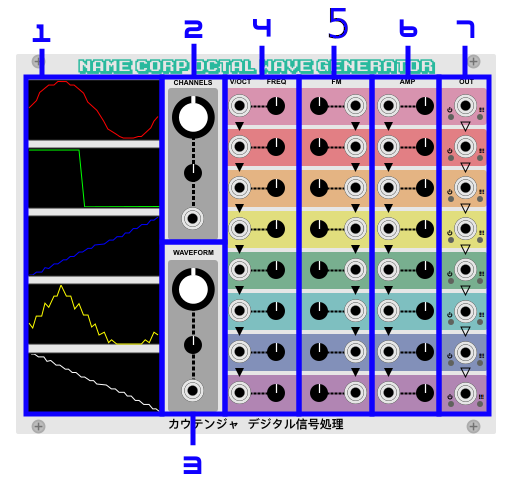
\includegraphics{Interface}
\end{figure}

\begin{enumerate}
  \item Waveform selection. Draw arbitrary waveforms using the mouse pointer.
  \item Channel selection. The big knob determine the number of oscillators in use by the chip. The small knob acts as an attenuverter for the linear CV input.
  \item Wave-table selection. The big knob determine the wave-table used by the chip. The small knob acts as an attenuverter for the linear CV input. Wave-table morphing is accomplished through 32-bit floating point linear interpolation.
  \item $V$/Octave inputs for the eight oscillators.
  \item CV linear frequency modulation for the eight oscillators.
  \item Coarse frequency control over the eight oscillators.
  \item CV linear amplitude modulation for the eight oscillators using the 4-bit amplifier.
  \item Coarse amplitude control over the eight oscillators using the 4-bit amplifier. When no input is connected, the slider controls the level from $0\%$ to $100\%$. When an input is connected, the slider acts as an attenuator.
  \item Channel outputs for the eight oscillators, ${\approx}10V_{pp}$. The LED indicates whether the oscillator is activated based on parameter (2). When in polyphonic mode, the lights become blue and display the average value of the light's brightness over the polyphonic channels.
\end{enumerate}

% -------------------
% MARK: References
% -------------------

\clearpage
\renewcommand\refname{References \& Acknowledgments}
\nocite{*}
\bibliographystyle{apalike}
\bibliography{references}

\end{document}
